% Options for packages loaded elsewhere
\PassOptionsToPackage{unicode}{hyperref}
\PassOptionsToPackage{hyphens}{url}
%
\documentclass[
]{book}
\usepackage{lmodern}
\usepackage{amssymb,amsmath}
\usepackage{ifxetex,ifluatex}
\ifnum 0\ifxetex 1\fi\ifluatex 1\fi=0 % if pdftex
  \usepackage[T1]{fontenc}
  \usepackage[utf8]{inputenc}
  \usepackage{textcomp} % provide euro and other symbols
\else % if luatex or xetex
  \usepackage{unicode-math}
  \defaultfontfeatures{Scale=MatchLowercase}
  \defaultfontfeatures[\rmfamily]{Ligatures=TeX,Scale=1}
\fi
% Use upquote if available, for straight quotes in verbatim environments
\IfFileExists{upquote.sty}{\usepackage{upquote}}{}
\IfFileExists{microtype.sty}{% use microtype if available
  \usepackage[]{microtype}
  \UseMicrotypeSet[protrusion]{basicmath} % disable protrusion for tt fonts
}{}
\makeatletter
\@ifundefined{KOMAClassName}{% if non-KOMA class
  \IfFileExists{parskip.sty}{%
    \usepackage{parskip}
  }{% else
    \setlength{\parindent}{0pt}
    \setlength{\parskip}{6pt plus 2pt minus 1pt}}
}{% if KOMA class
  \KOMAoptions{parskip=half}}
\makeatother
\usepackage{xcolor}
\IfFileExists{xurl.sty}{\usepackage{xurl}}{} % add URL line breaks if available
\IfFileExists{bookmark.sty}{\usepackage{bookmark}}{\usepackage{hyperref}}
\hypersetup{
  pdftitle={DBG0061 - Portfólio},
  pdfauthor={João Vitor Ferreira Cavalcante},
  hidelinks,
  pdfcreator={LaTeX via pandoc}}
\urlstyle{same} % disable monospaced font for URLs
\usepackage{longtable,booktabs}
% Correct order of tables after \paragraph or \subparagraph
\usepackage{etoolbox}
\makeatletter
\patchcmd\longtable{\par}{\if@noskipsec\mbox{}\fi\par}{}{}
\makeatother
% Allow footnotes in longtable head/foot
\IfFileExists{footnotehyper.sty}{\usepackage{footnotehyper}}{\usepackage{footnote}}
\makesavenoteenv{longtable}
\usepackage{graphicx,grffile}
\makeatletter
\def\maxwidth{\ifdim\Gin@nat@width>\linewidth\linewidth\else\Gin@nat@width\fi}
\def\maxheight{\ifdim\Gin@nat@height>\textheight\textheight\else\Gin@nat@height\fi}
\makeatother
% Scale images if necessary, so that they will not overflow the page
% margins by default, and it is still possible to overwrite the defaults
% using explicit options in \includegraphics[width, height, ...]{}
\setkeys{Gin}{width=\maxwidth,height=\maxheight,keepaspectratio}
% Set default figure placement to htbp
\makeatletter
\def\fps@figure{htbp}
\makeatother
\setlength{\emergencystretch}{3em} % prevent overfull lines
\providecommand{\tightlist}{%
  \setlength{\itemsep}{0pt}\setlength{\parskip}{0pt}}
\setcounter{secnumdepth}{5}
\usepackage[utf8]{inputenc}
\usepackage[portuguese]{babel}
\usepackage{booktabs}
\usepackage{amsthm}
\makeatletter
\def\thm@space@setup{%
  \thm@preskip=8pt plus 2pt minus 4pt
  \thm@postskip=\thm@preskip
}
\makeatother
\usepackage[]{natbib}
\bibliographystyle{apalike}

\title{DBG0061 - Portfólio}
\author{João Vitor Ferreira Cavalcante}
\date{2020-06-23}

\begin{document}
\maketitle

{
\setcounter{tocdepth}{1}
\tableofcontents
}
\hypertarget{prefuxe1cio}{%
\chapter{Prefácio}\label{prefuxe1cio}}

Esse é o meu portfólio para a disciplina DBG0061 - RNAs Não Codantes, cursada no semestre suplementar 2020.5.

Aqui estarão contidas respostas para os exercícios de cada dia, dúvidas e reflexões sobre os seminários.

As duas principais referências usadas foram os encontros de cada aula e o livro ``Introdução ao universo dos non-coding RNAs'' de Tiago Campos Pereira. Fontes alternativas, se utilizadas, são citadas em cada capítulo.

\hypertarget{aula1}{%
\chapter{mRNA, tRNA e rRNA}\label{aula1}}

\hypertarget{identifique-as-funuxe7uxf5es-de-cada-um}{%
\section{Identifique as funções de cada um}\label{identifique-as-funuxe7uxf5es-de-cada-um}}

\begin{itemize}
\item
  O mRNA é o responsável por carregar a informação codante do genoma, gerado no processo de transcrição,
  ele é o passo inicial para a produção de proteínas.
\item
  O tRNA é aquele que irá interpretar a informação contida no mRNA processado, se ligando aos seus códons e trazendo consigo o respectivo aminoácido.
\item
  O rRNA, por fim, será aquele responsável pela consolidação final da informação proteica, ao trafegar pelo mRNA, indica quais tRNAs devem se ligar e une os seus respectivos aminoácidos para a formação da proteína.
\end{itemize}

\hypertarget{regioes}{%
\section{Nomeie as regiões de um RNA mensageiro}\label{regioes}}

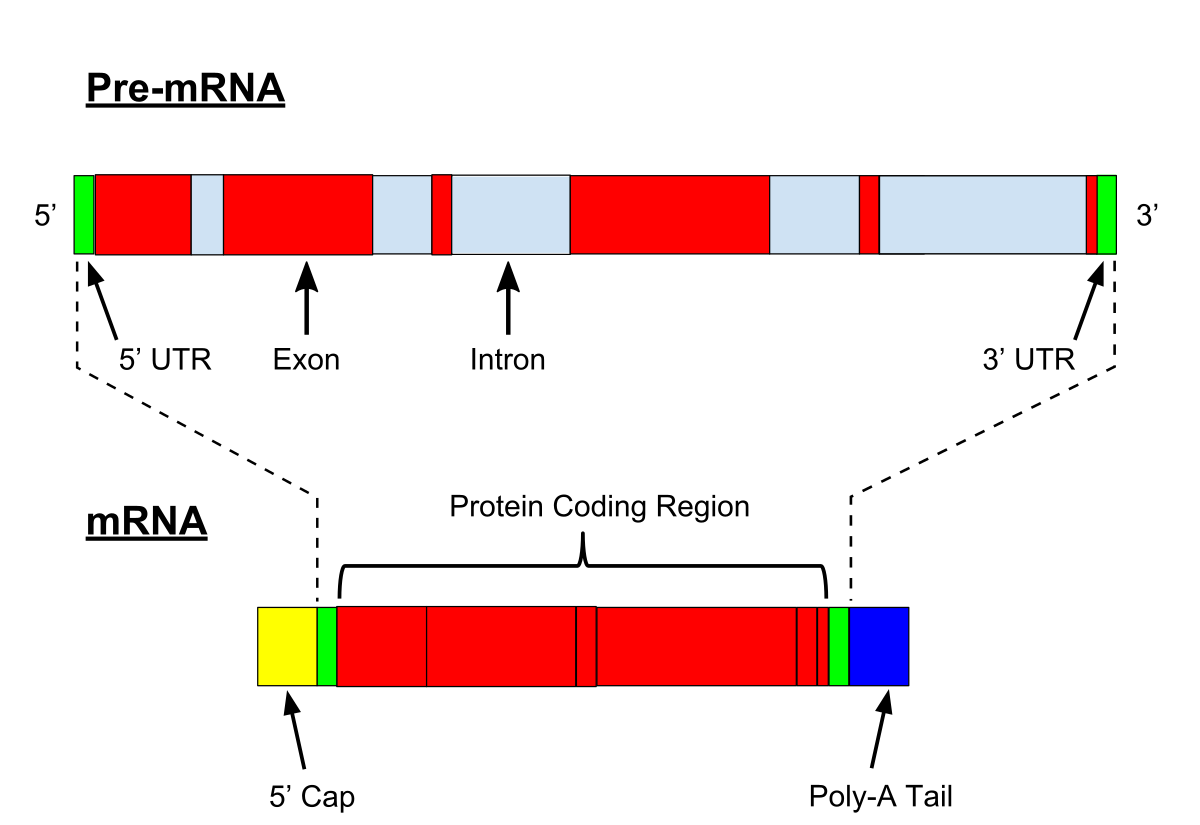
\includegraphics{./pics/estruturamrna.png}

Inicialmente, o mRNA possui 3 principais componentes: Os íntrons, que não codificam a informação proteica final, os éxons, a porção codante, e as UTRs em cada ponta, que são, também, regiões não traduzidas. Após o processamento, observa-se a adição de um ``capacete'' na extremidade 5' e uma sequência poli-A na extremidade 3', ambas estruturas que auxiliam na proteção do mRNA de exonucleases.

\hypertarget{gerauxe7uxe3o-e-modificauxe7uxf5es-puxf3s-transcricionais}{%
\section{Geração e modificações pós-transcricionais}\label{gerauxe7uxe3o-e-modificauxe7uxf5es-puxf3s-transcricionais}}

\hypertarget{mrna}{%
\subsection{mRNA}\label{mrna}}

A \textbf{transcrição}, em eucariotos, ocorre por meio da RNA Polimerase II, que junto a um ou mais fatores de transcrição, se liga
ao promotor, formando a bolha de transcrição, posteriormente, à medida que as ligações de hidrogênio vão sendo quebradas pela forquilha, vai se formando a fita, com a adição de nucleotídeos de RNA complementares. Ao fim deste processo teremos o pre-mRNA, que passará pelo processamento mencionado em \ref{regioes}

\hypertarget{trna}{%
\subsection{tRNA}\label{trna}}

Seus genes, localizados no nucléolo, são transcritos pela RNA Polimerase III. Em seguida ocorre o processamento do pre-tRNA formado, iniciando com a remoção de certas sequências, tanto na ponta 3' quanto na 5'. Vale destacar que inicialmente alguns tRNAs possuem íntrons, que em procariotos se auto-removem, mas em eucariotos e arqueas são removidos por endonucleases, que reconhecem sua região BHB. Por fim, há a adição de CCA na sua extremidade 3', posteriormente a isso o tRNA ainda pode passar por diversos processamentos, a depender do aminoácido ao qual se relaciona.

E, ultimamente, é claro, há a reação de aminoacilação quando o tRNA for executar sua função na célula.

\hypertarget{rrna}{%
\subsection{rRNA}\label{rrna}}

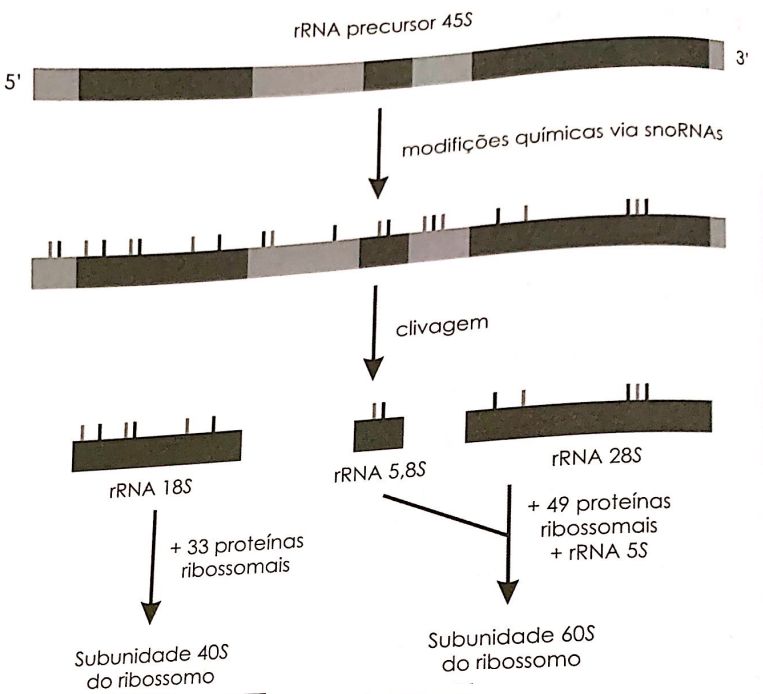
\includegraphics{./pics/rRNA synthesis.png}

Em eucariotos, ocorre no nucléolo, com a síntese do 45S pela RNA Polimerase I, este possuinte de regiões interespaçadas transcritas que assemelham íntrons, e no núcleo, com a síntese do 5S pela RNA Polimerase III. O 45S, após passar por modificações realizadas por snoRNAs, como metilação e pseudouridilação, tem seus espaçadores clivados. Os fragmentos resultantes se unem a proteínas ribossomais, formando as duas subunidades conhecidas, a 40S e a 60S.

\hypertarget{ediuxe7uxe3o-de-rna}{%
\section{Edição de RNA}\label{ediuxe7uxe3o-de-rna}}

É o processo no qual ocorrem modificações no RNA que não refletem mutações na sequência genômica original. Essas modificações podem ser inserções, deleções e substituições. Algumas modificações de nota são:

\begin{itemize}
\item
  Edição do gene da ApoB - uma troca de C para U - reflete nas isoformas observadas da proteína no organismo, a ApoB-100 (hepática) e a ApoB-48 (intestinal), essa última que possui seu tamanho reduzido pois a troca gera um códon de parada.
\item
  Conversão de A para Inosina pela \textbf{ADAR} em miRNAs, que pode impedir o processamento por DROSHA e DICER.
\end{itemize}

\hypertarget{primers-de-rna}{%
\chapter{Primers de RNA}\label{primers-de-rna}}

\hypertarget{o-que-suxe3o}{%
\section{O que são?}\label{o-que-suxe3o}}

São pequenas sequências nucleotídicas de fita única, responsáveis pela iniciação da síntese de uma sequência nucleotídica maior,
como ocorre na síntese de DNA.

\hypertarget{como-suxe3o-gerados}{%
\section{Como são gerados?}\label{como-suxe3o-gerados}}

São gerados pela primase, que se acopla à fita de DNA quando ligada a uma molécula de ATP, formando inicialmente um dinucleotídeo pppApG ligado à seu ATP, em seguida organiza os nucleotídeos restantes do primer pela sua complementaridade com o DNA.

\hypertarget{onde-suxe3o-usados}{%
\section{Onde são usados?}\label{onde-suxe3o-usados}}

São usados na síntese de DNA, como falado anteriomente, visto que as DNAs polimerases não tem capacidade de iniciar o processo sozinhas. Mas também são usados na transcrição reversa, como é o caso da Telomerase em humanos, em que seu componente TERC é fundamental, auxiliando na manutenção da longevidade da molécula de DNA.

E, é claro, possuem inúmeras aplicações na biologia molecular, destacando-se as principais técnicas usadas nessa área, o PCR e o Sequenciamento, para as quais os primers são indispensáveis.

\hypertarget{qual-a-importuxe2ncia-deles-pros-retrovuxedrus}{%
\section{Qual a importância deles pros retrovírus?}\label{qual-a-importuxe2ncia-deles-pros-retrovuxedrus}}

Os primers de RNA são fundamentais para a replicação dos retrovírus, visto que, como o próprio nome diz, esses vírus utilizam um molde de RNA para sintetizar DNA, o início do processo se dá com um primer. Este primer, que muitas vezes é um tRNA de lisidina, se acopla à seção do genoma viral chamado de PBS, o que possibilita o início da polimerização pela Transcriptase Reversa, adicionando-se nucleotídeos na extremidade 3' do primer. Após a degradação de seções não codantes e repetitivas na extremidade 3' o primer de tRNA se desloca para a extremidade 5', extendendo a nova fita de DNA nesse sentido.

\hypertarget{snrna-e-snorna}{%
\chapter{snRNA e snoRNA}\label{snrna-e-snorna}}

\hypertarget{o-que-suxe3o-ribonucleoproteuxednas}{%
\section{O que são ribonucleoproteínas?}\label{o-que-suxe3o-ribonucleoproteuxednas}}

São complexos formados por ácidos ribonucléicos e RBPs ou proteínas de ligação a RNA,
alguns exemplos são os ribossomos e os snRNPs, estes últimos formados pela associação de snRNAs a proteínas, preenchendo funções de extrema relevância para o processo de splicing.

\hypertarget{descriuxe7uxf5es-desses-dois-ncrnas}{%
\section{Descrições desses dois ncRNAs}\label{descriuxe7uxf5es-desses-dois-ncrnas}}

\hypertarget{snrnas}{%
\subsection{snRNAs}\label{snrnas}}

São pequenos RNAs sintetizados no núcleo, especificamente nos corpos de Cajal, possuem um comprimento médio de 150nt e podem ser transcritos tanto pela RNAPol-II quanto pela RNAPol-III. Preenchem funções relevantes no processo de splicing. Se tem conhecimento de por volta de 10 snRNAs e estes são divididos em duas classes:

\begin{itemize}
\item
  Os Sm, transcritos pela RNAPol-II, são exportados para o citoplasma, onde sofrem clivagem na extremidade 3' resultando na formação de um loop. A estrutura em loop 3' é necessária para o reconhecimento pela proteína SMN, que proporcionará a hipermetilação de seu cap 5', originando um cap de tri-metilguanosina, que é necessário para seu endereçamento celular para os corpúsculos de Cajal, onde podem passar por pseudouridinilações e mais metilações.
\item
  Os Lsm, transcritos pela RNAPol-III, possuindo um cap 5' de monometilfosfato, nunca deixam o núcleo, se ligando a proteína La, o que proporciona a ligação do anel Lsm, o que indica seu endereçamento para o nucléolo, onde por fim pode passar pelas pseudouridinilações e metilações que o farão funcional.
\end{itemize}

\hypertarget{snornas}{%
\subsection{snoRNAs}\label{snornas}}

São pequenos RNAs localizados no nucléolo, podendo se maturar nele mesmo ou nos corpúsculos de Cajal. Tem tamanho variando de 60 a 170nt. São, em sua grande parte, transcritos
pela RNAPol-II. Se dividem, também, em duas classes, diferenciando-se pelos boxes, ou sequências curtas conservadas, que possuem:

\begin{itemize}
\item
  Os box H/ACA possuem duas estruturas secundárias interceptadas por um box H e um box ACA.
\item
  Os box C/D possuem pareamentos nas suas extremidades, onde são localizados os dois boxes, C e D.
\end{itemize}

\hypertarget{onde-eles-atuam}{%
\section{Onde eles atuam?}\label{onde-eles-atuam}}

\hypertarget{snrnas-1}{%
\subsection{snRNAs}\label{snrnas-1}}

A grande maioria participa do spliceossomo (Abaixo descreve-se splicing U2):

\begin{itemize}
\item
  Inicialmente, há a ligação do complexo U1 ao sítio de splicing 5', mediada pela complementaridade do snRNA que possui.
\item
  Logo em seguida, ocorre a ligação do complexo U2 ao ponto de ramificação do íntron.
\item
  As reações de transestefiricação subsequentes, propiciadas inicialmente pela hidroxila 2 do ponto de ramificação, irão resultar na ligação dos éxons adjacentes e a liberação do íntron na forma de laço.
\end{itemize}

\hypertarget{snornas-1}{%
\subsection{snoRNAs}\label{snornas-1}}

Formam os complexos de snoRNPs, com as porções ribonucleotídicas agindo como um ``guia'', indicando seções nos rRNAs não processados e, com o pareamento destes, proporcionam reações de metilação e pseudouridinilação, estas necessárias para a clivagem e formação da estrutura final do ribossomo.

\hypertarget{a-quais-doenuxe7as-estuxe3o-relacionados}{%
\section{A quais doenças estão relacionados?}\label{a-quais-doenuxe7as-estuxe3o-relacionados}}

\hypertarget{snrnas-2}{%
\subsection{snRNAs}\label{snrnas-2}}

\begin{itemize}
\item
  \textbf{Atrofia muscular espinhal}: Mutações no SMN que podem resultar na perda da função das suas proteínas, com sua responsabilidade na síntese dos snRNAs Sm sendo prejudicada.
\item
  \textbf{Medulloblastoma}: Alguns desses tumores possuem um U1 snRNA mutado, o que leva a alterações negativas no splicing.
\end{itemize}

\hypertarget{snornas-2}{%
\subsection{snoRNAs}\label{snornas-2}}

\begin{itemize}
\item
  \textbf{Síndrome de Prader-Willi}: Foi observado que perdas de cópias do SNORD116 está associado ao surgimento dessa síndrome \citep{Sahoo_2008}.
\item
  \textbf{Autismo}: Ganho de cópias do SNORD115 pode estar associado ao surgimento de algumas formas de autismo \citep{Bolton_2004}
\end{itemize}

\hypertarget{histuxf3rico-dos-mirnas}{%
\chapter{Histórico dos miRNAs}\label{histuxf3rico-dos-mirnas}}

\hypertarget{qual-foi-o-primeiro-mirna-e-como-ele-foi-identificado}{%
\section{Qual foi o primeiro miRNA e como ele foi identificado?}\label{qual-foi-o-primeiro-mirna-e-como-ele-foi-identificado}}

\begin{figure}
\centering
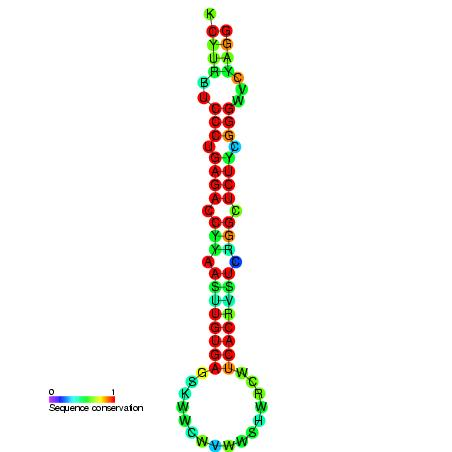
\includegraphics{./pics/lin4.jpg}
\caption{(Rfam database)}
\end{figure}

O lin-4 foi descoberto em um experimento que pretendia elucidar funções de genes heterocrônicos do \emph{C. elegans}, inicialmente, se foi observado que na diferenciação dos estágios de vida L1 e L2, havia aumento do RNA lin-4 e diminuição da \textbf{proteína} lin-14, porém isso não se refletia numa diminuição dos transcritos de lin-14, o que indica uma regulação negativa pós-transcricional. Foi observado, posteriormente, que essa regulação estava associada com a região 3' UTR do lin-14.

\hypertarget{que-alvos-ele-controla}{%
\section{Que alvos ele controla?}\label{que-alvos-ele-controla}}

Regula negativamente a tradução da proteína lin-14, o que possibilita o desenvolvimento adequado do \emph{C. elegans} em seus estágios larvais. Posteriormente também foi descoberto que ele regula negativamente o lin-28.

\hypertarget{qual-seu-mecanismo-de-auxe7uxe3o}{%
\section{Qual seu mecanismo de ação;}\label{qual-seu-mecanismo-de-auxe7uxe3o}}

Ele pareia com a região 3' UTR do lin-14, alterando o prosseguimento da tradução - impedindo a finalização ou prolongamento desta.

\hypertarget{identificar-e-comentar-as-3-outras-descobertas-importantes-sobre-os-mirnas}{%
\section{Identificar e comentar as 3 outras descobertas importantes sobre os miRNAs}\label{identificar-e-comentar-as-3-outras-descobertas-importantes-sobre-os-mirnas}}

\begin{itemize}
\item
  Descobertas anteriores sobre a capacidade de RNAs antisenso de afetarem a estabilidade e alterarem a tradução de RNAs mensageiros.
\item
  A descoberta de que o lin-14 não atua impedindo o início da tradução, atuando posteriormente ao início, inclusive podendo atuar em mais de uma etapa diferente.
\item
  A descoberta do segundo miRNA, o let-7, que regula negativamente o lin-41, também importante no desenvolvimento do \emph{C. elegans}, porém agora na transição para o estágio L4.
\end{itemize}

\hypertarget{ideias-gerais-de-3-artigos-seminais}{%
\section{Ideias gerais de 3 artigos seminais}\label{ideias-gerais-de-3-artigos-seminais}}

\begin{itemize}
\item
  \citep{Lau_2001} miRNAs podem ser transcritos na forma de cluster. Também podendo ser co-expressos durante a embriogênese. Porém, talvez mais relevante, a existência de ortólogos potenciais dos genes de miRNA em humanos.
\item
  \citep{Lagos_Quintana_2001} Isolamento de miRNAs em \emph{Drosophila} e células HeLa. Identificando-se 21 miRNAs diferentes em humano.
\item
  \citep{Lee_2001} Descoberta de vários novos miRNAs em \emph{C. elegans} indicando também possíveis homólogos no ser humano.
\end{itemize}

\hypertarget{referuxeancias}{%
\chapter{Referências}\label{referuxeancias}}

  \bibliography{book.bib}

\end{document}
